% Include Preamble 
\documentclass[10pt,dvipsnames, aspectratio=169]{beamer}
\usetheme[progressbar=frametitle]{metropolis}
\usepackage[]{verbatim}\usepackage[]{}
\usepackage{booktabs}
\usepackage[scale=2]{ccicons}
\usepackage[misc]{ifsym}
\usepackage{wasysym}
\usepackage{listings}
\usepackage{xspace}
\usepackage{amsmath}
\usepackage{xcolor}
\usepackage{ragged2e}\justifying % for justify content % Customize 
\setlength{\parskip}{5pt} % vertical spacing between 2 paragraphs
\setbeamersize{text margin left=12mm, text margin right=12mm} 
\setbeamertemplate{frametitle}[default][left, leftskip=8mm]
%\usepackage[hidelink]{hyperref}
\newcommand{\themename}{\textbf{\textsc{metropolis}}\xspace}

% WARNING: Don't Touch,if you are not compfortable! 
\addtobeamertemplate{frametitle}{}{
%\begin{tikzpicture}[remember picture,overlay]
%\node[anchor=north east,yshift=2pt,xshift=-65pt] at (current page.north east) 
%{\includegraphics[height=.75cm]{img/elixir-portugal-white}};
%\node[anchor=north east,yshift=4pt] at (current page.north east) 
%{
\includegraphics[height=1cm]{img/hdro}};
%\end{tikzpicture}
}

% Title Page of Presentation 
% WARNING: Don't change logo, just write your details 
\title{Introduction to SPSS}
\date{\today}
\author{Md. Jubayer Hossain\\
        https://jhossain.me/}
\institute{Lead Organizer, Health Research ToolBox: A Step by Step Guide for Beginners 
\\ Founder,Center for Health Innovation, Research, Action, and Learning }
\titlegraphic{\vspace{4cm}\hfill
\includegraphics[height=1cm]{img/hdro2}}
\begin{document}

\maketitle
% Sectuion Title 
\section{SECTION--I Summary Statistics for Individual Variable}
%-------------------Summary Measures for Categorical Data-------------------------
% Slide 
\begin{frame}[t]{Summary Measures for Categorical Data (Con..)}
	\begin{itemize}
		\item From the menus choose:\\
		Analyze \textgreater Descriptive Statistics \textgreater Frequencies...\\
		\item Select Glucose and BloodPressure and move them into the Variable(s) list.
		\item Click OK to run the procedure.
	\end{itemize}
	
\end{frame}
% Slide 
\begin{frame}[t]{Summary Measures for Categorical Data (Con..)}
	\begin{figure}
		\centering
		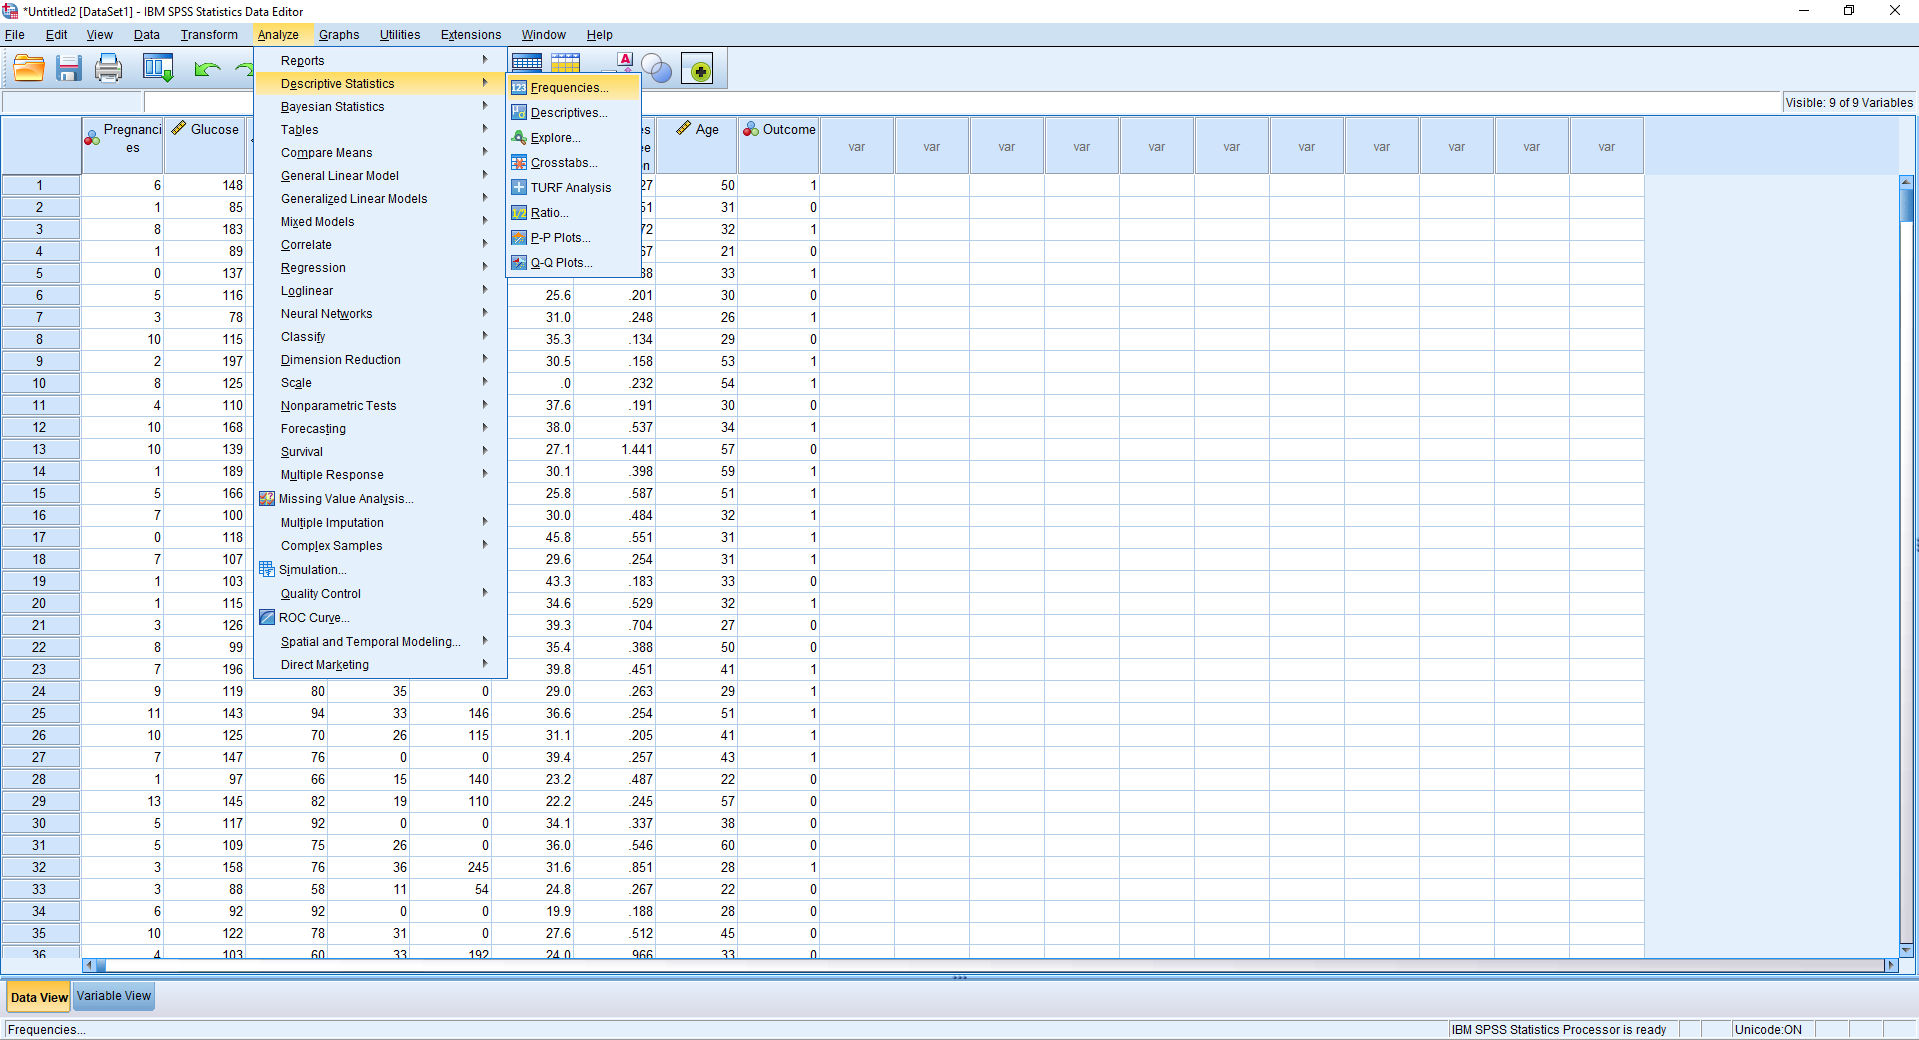
\includegraphics[width=12cm]{img/freq_table1_1}
	\end{figure}
\end{frame}
% Slide 
\begin{frame}[t]{Summary Measures for Categorical Data (Con..)}
	\begin{figure}
		\centering
		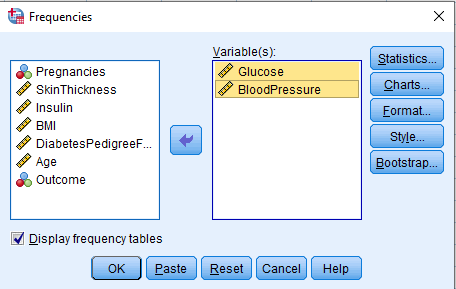
\includegraphics[width=10cm]{img/freq_table1_2}
		\caption{Click Ok}
	\end{figure}
\end{frame}
% Slide 
\begin{frame}[t]{Summary Measures for Categorical Data}
	\begin{figure}
		\centering
		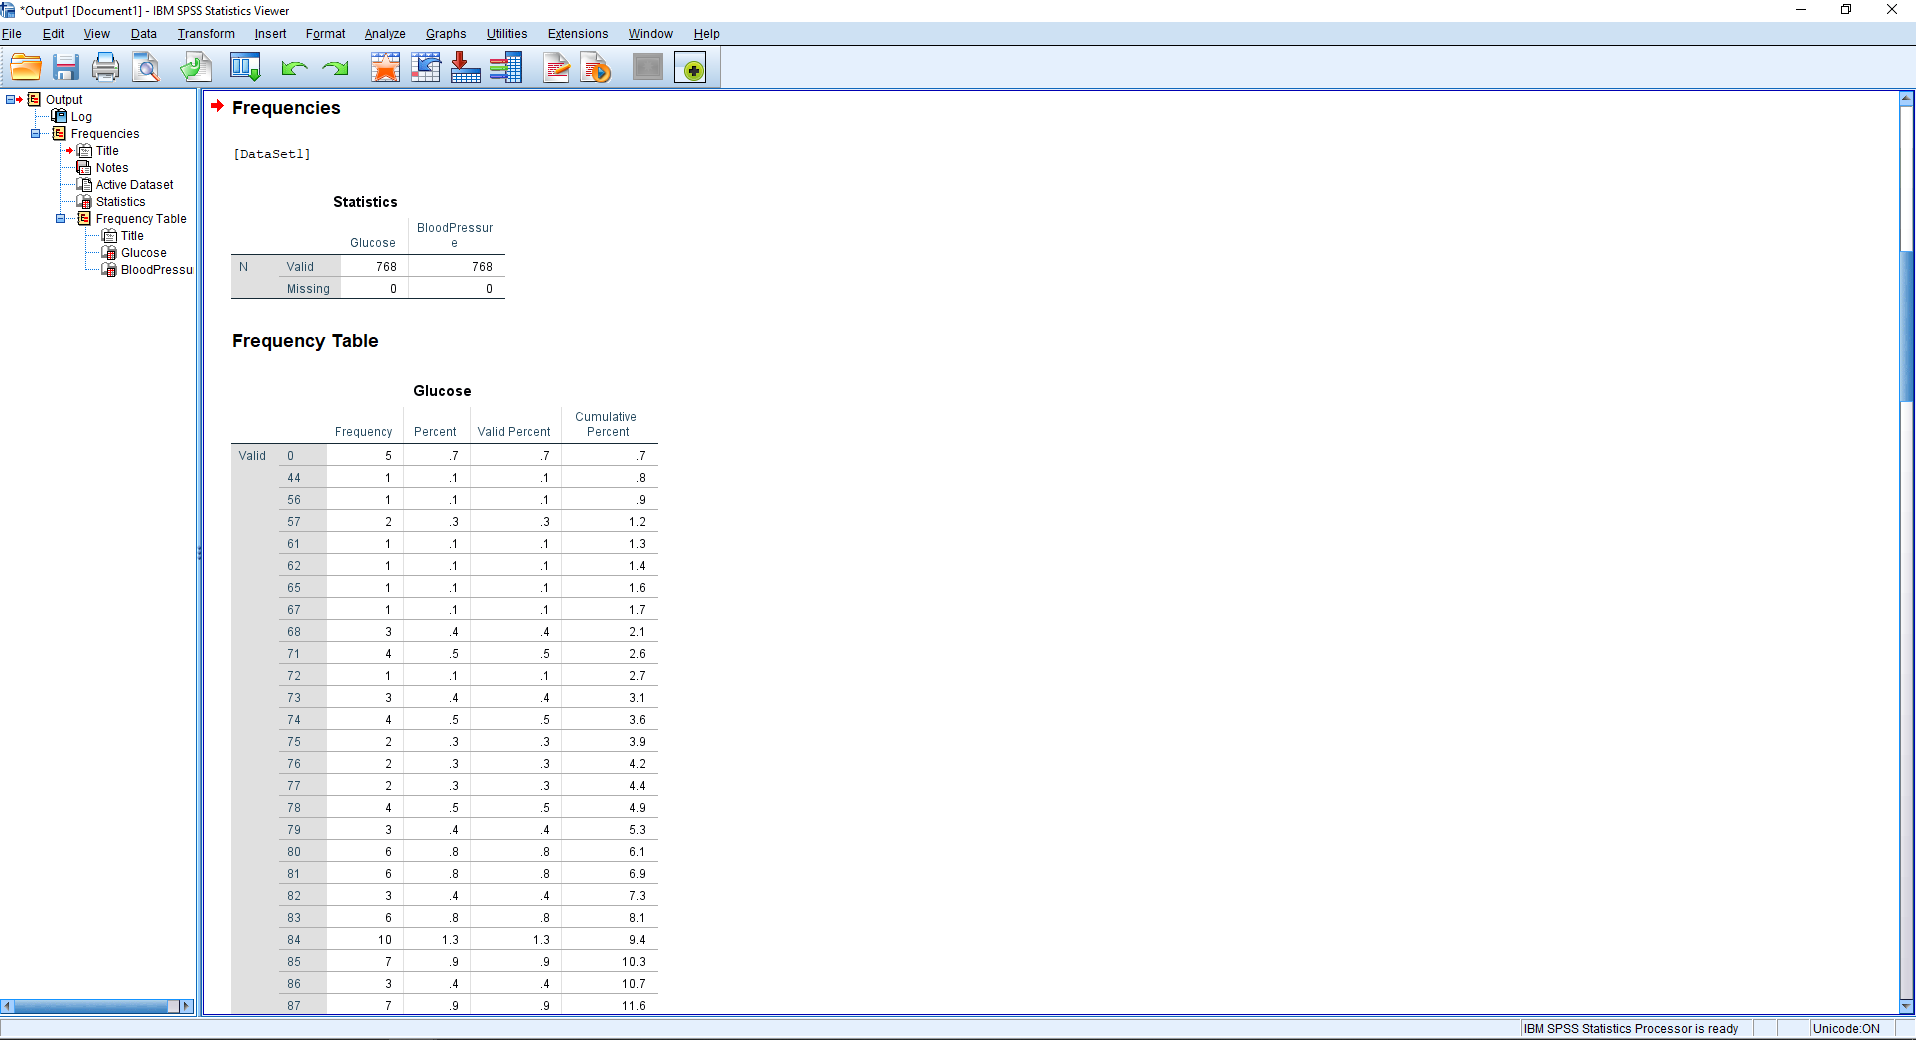
\includegraphics[width=12cm]{img/freq_table1_3}
	\end{figure}
\end{frame}
%-------------------End-------------------------


%-------------------Charts for Categorical Data-------------------------
%slide
\begin{frame}[t]{Charts for Categorical Data (Con..)}
	 \begin{itemize}
	 	\item Open the Frequencies dialog box again.
	 	\item Click Charts.
	 	\item Select Bar charts and then click Continue.
	 	\item Click Ok.
	 \end{itemize}
\end{frame}
% Slide 
\begin{frame}[t]{Charts for Categorical Data (Con..)}
	\begin{figure}
		\centering
		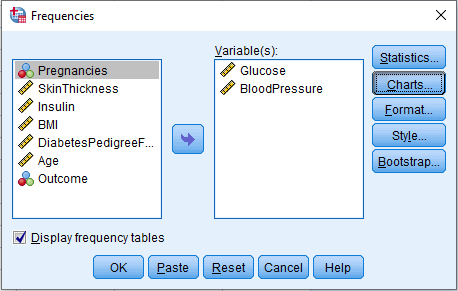
\includegraphics[width=10cm]{img/freq_charts_1}
		\caption{Click Ok}
	\end{figure}
\end{frame}
% Slide 
\begin{frame}[t]{Charts for Categorical Data (Con..)}
	\begin{figure}
		\centering
		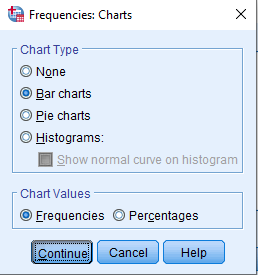
\includegraphics[width=5cm]{img/freq_charts_2}
	\end{figure}
\end{frame}
% Slide 
\begin{frame}[t]{Charts for Categorical Data (Con..)}
	\begin{figure}
		\centering
		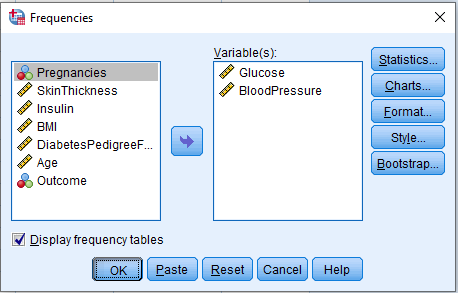
\includegraphics[width=10cm]{img/freq_charts_3}
		\caption{Click Ok}
	\end{figure}
\end{frame}
% Slide 
\begin{frame}[t]{Charts for Categorical Data}
	\begin{figure}
		\centering
		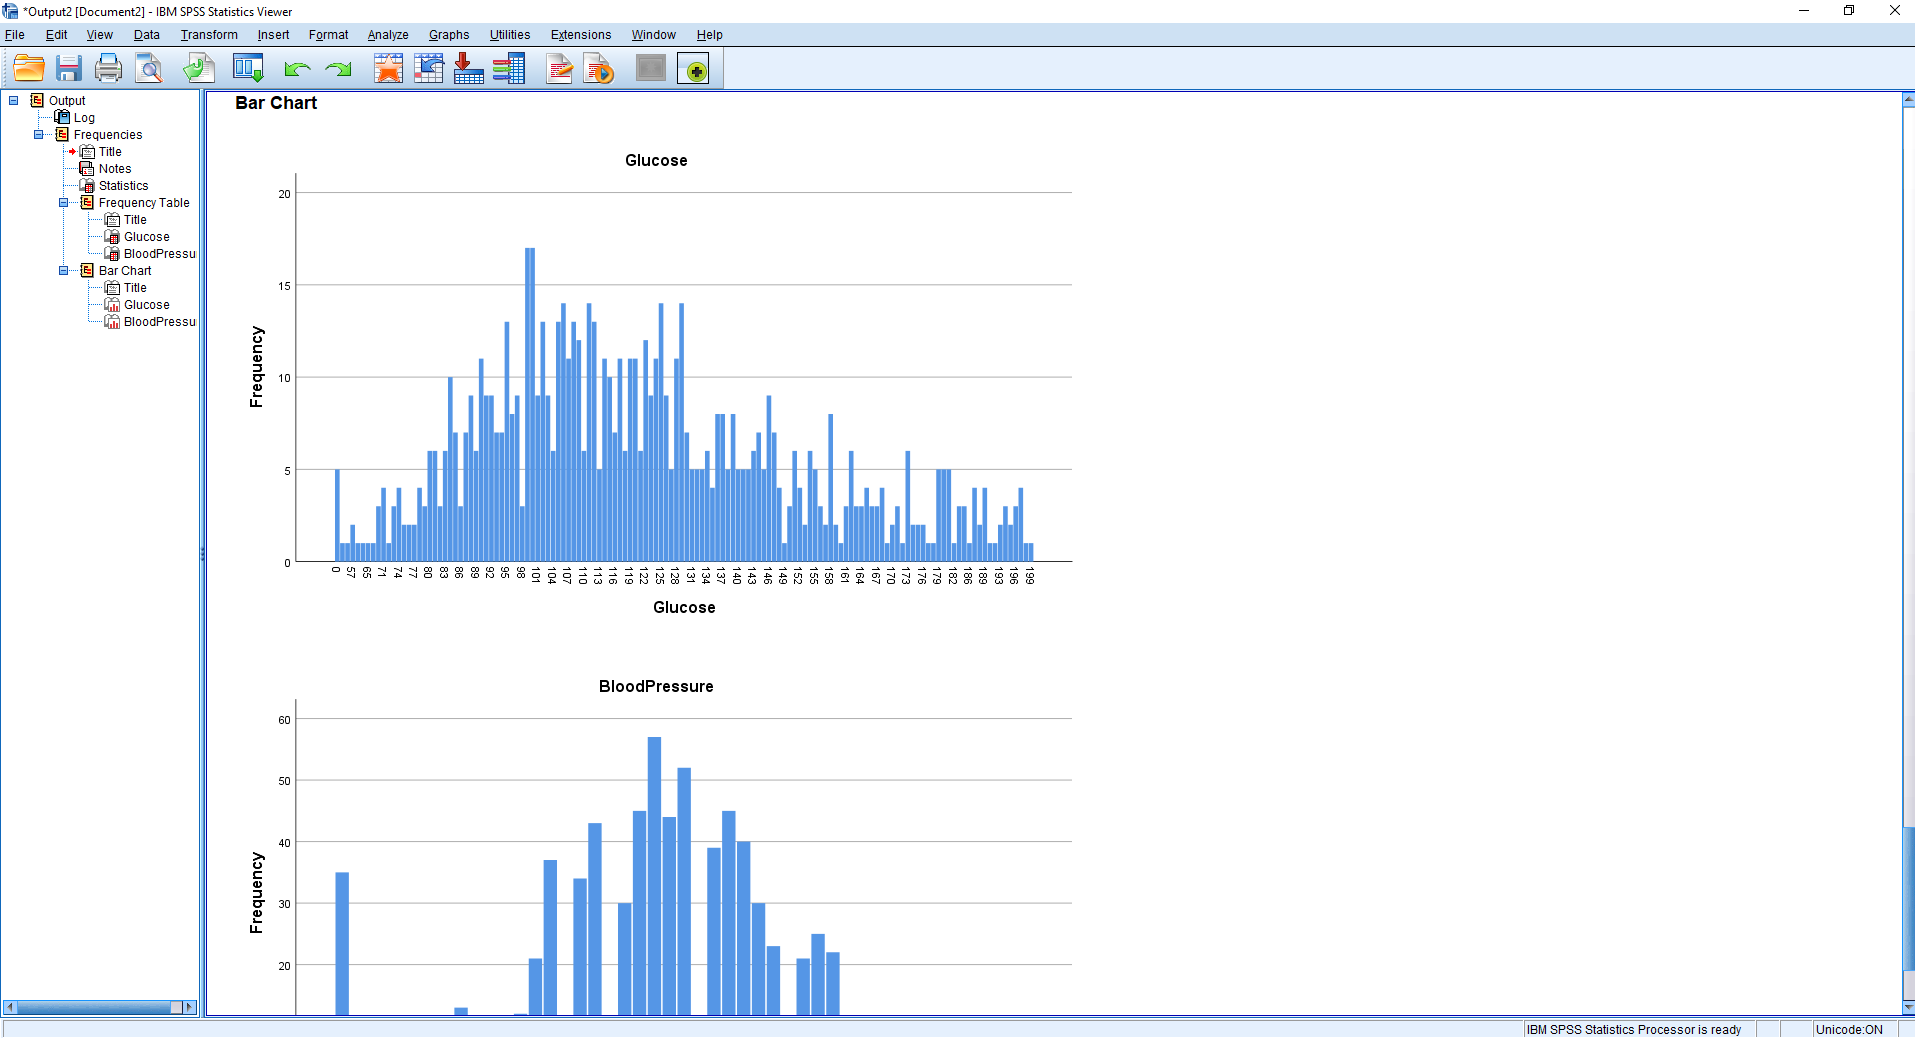
\includegraphics[width=12cm]{img/freq_charts_4}
		\caption{Result}
	\end{figure}
\end{frame}
%-----------------------End----------------------------------


%-------------------Summary Measures for Scale Variables-------------------------
%slide
\begin{frame}[t]{Summary Measures for Scale Variables (Con..)}
	\begin{itemize}
		\item Open the Frequencies dialog box again.
		\item Click Reset to clear any previous settings.
		\item Select BMI and move it into the Variable(s) list.
		\item Click Statistics.
		\item Select Mean, Median, Std. deviation, Minimum, and Maximum.
		\item Click Continue.
	\end{itemize}
\end{frame}
% Slide 
\begin{frame}[t]{Summary Measures for Scale Variables (Con..)}
	\begin{figure}
		\centering
		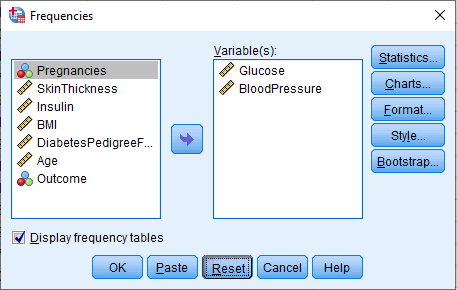
\includegraphics[width=10cm]{img/1111111}
		\caption{Click Reset}
	\end{figure}
\end{frame}
% Slide 
\begin{frame}[t]{Summary Measures for Scale Variables (Con..)}
	\begin{figure}
		\centering
		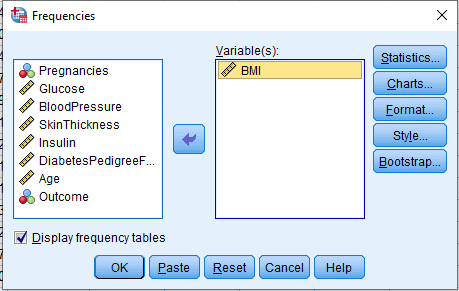
\includegraphics[width=8cm]{img/1111112}
		/
		\caption{Select BMI}
	\end{figure}
\end{frame}
% Slide 
\begin{frame}[t]{Summary Measures for Scale Variables (Con..)}
	\begin{figure}
		\centering
		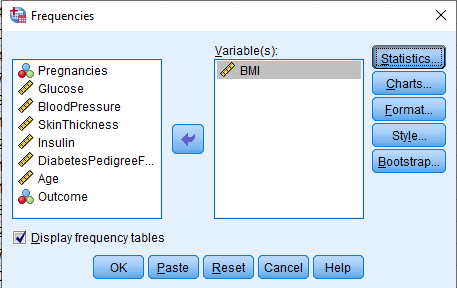
\includegraphics[width=8cm]{img/1111113}
		\caption{Click Statistics}
	\end{figure}
\end{frame}
% Slide 
\begin{frame}[t]{Summary Measures for Scale Variables (Con..)}
	\begin{figure}
		\centering
		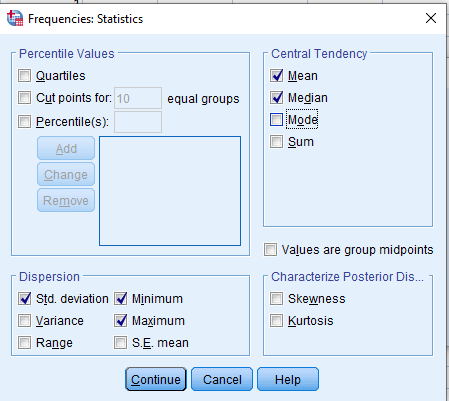
\includegraphics[width=6cm]{img/1111114}
		\caption{Select necessary Statistic options}
	\end{figure}
\end{frame}
% Slide 
\begin{frame}[t]{Summary Measures for Scale Variables (Con..)}
	\begin{figure}
		\centering
		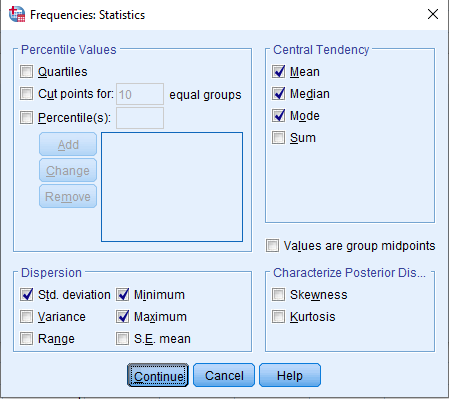
\includegraphics[width=6cm]{img/1111115}
		\caption{Click Continue}
	\end{figure}
\end{frame}
% Slide 
\begin{frame}[t]{Summary Measures for Scale Variables}
	\begin{figure}
		\centering
		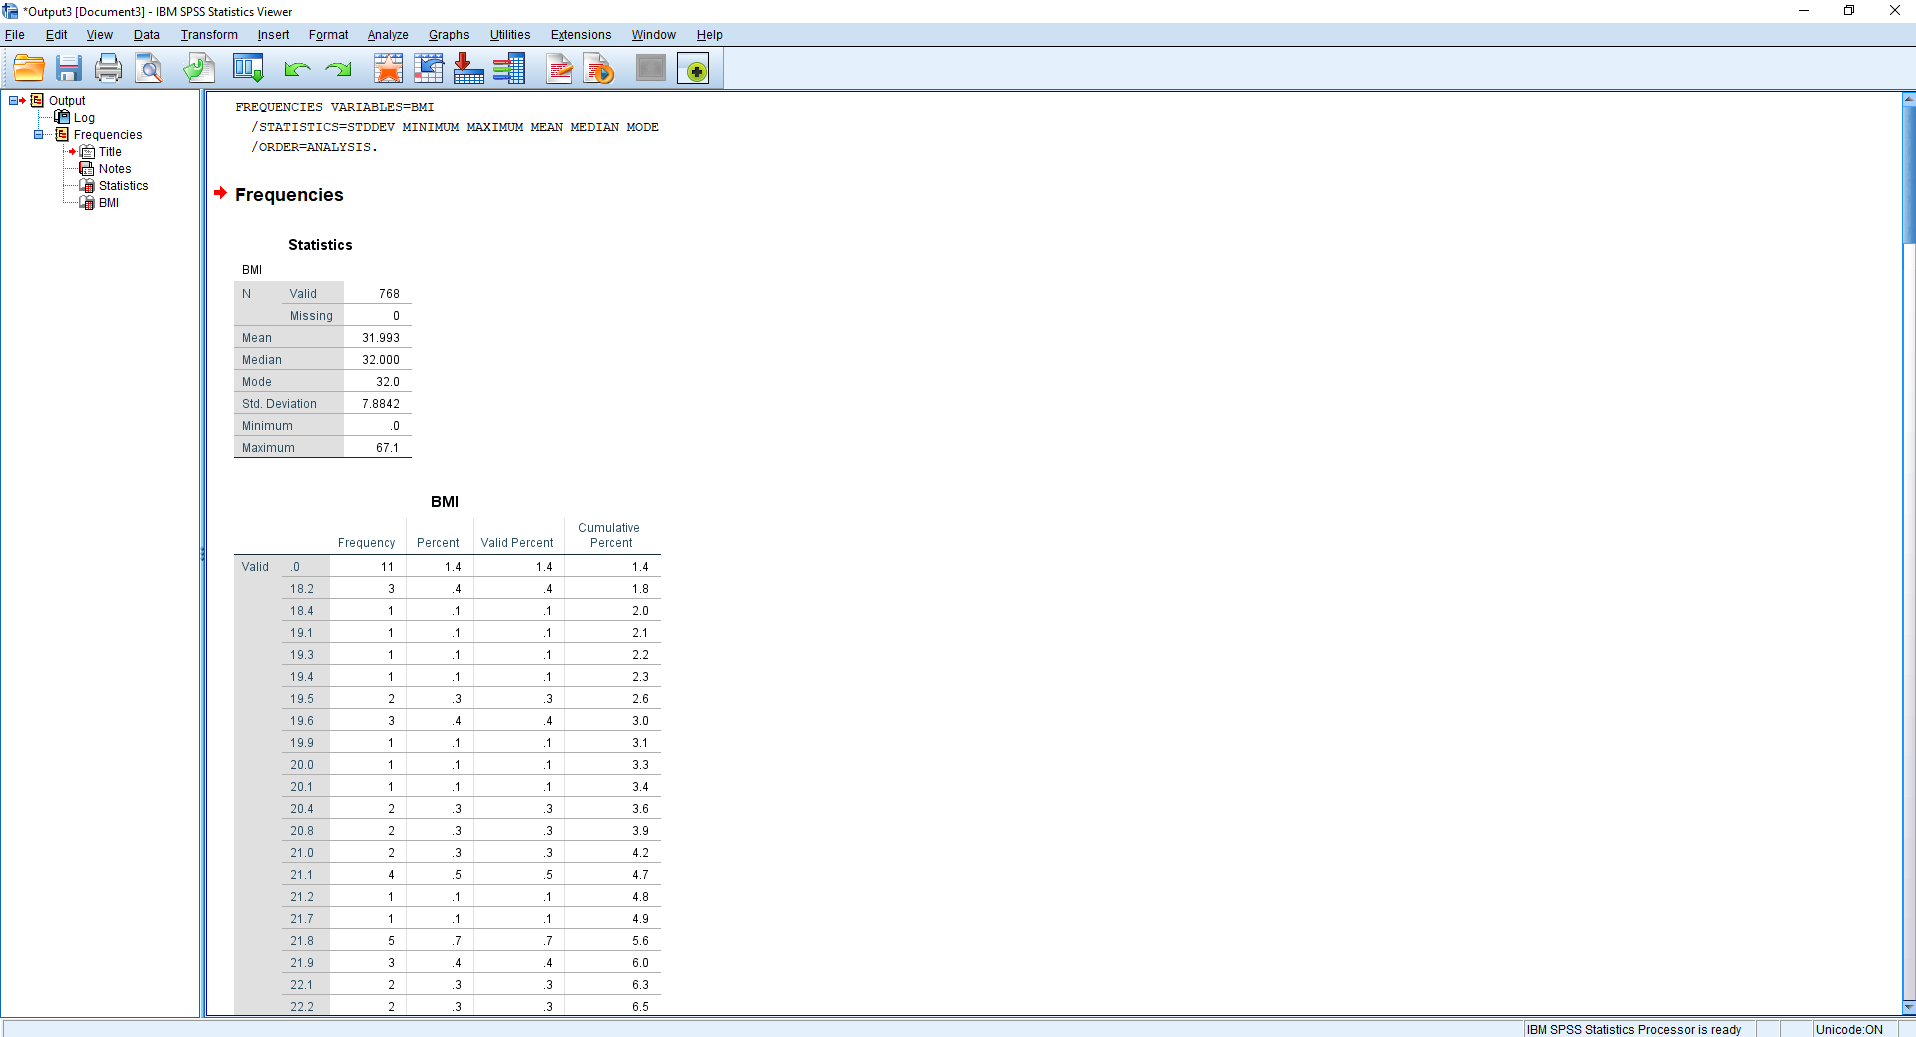
\includegraphics[width=12cm]{img/1111116}
		\caption{Result}
	\end{figure}
\end{frame}
%-----------------------End----------------------------------



%-------------------Charts for Categorical Data-------------------------
%slide
\begin{frame}[t]{Histograms for Scale Variables (Con..)}
	\begin{itemize}
		\item Open the Frequencies dialog box again.	
		\item Click Charts.
		\item Select Histograms and With normal curve.
		\item Click Continue, and then click OK in the main dialog box to run the procedure.
		
	\end{itemize}
\end{frame}
% Slide 

% Slide 
\begin{frame}[t]{Histograms for Scale Variables (Con..)}
	\begin{figure}
		\centering
		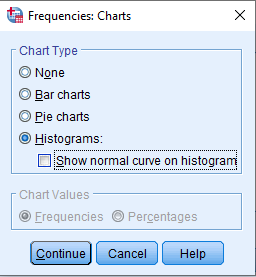
\includegraphics[width=6cm]{img/1111117}
		\caption{Click Histograms}
	\end{figure}
\end{frame}
% Slide 
\begin{frame}[t]{Histograms for Scale Variables (Con..)}
	\begin{figure}
		\centering
		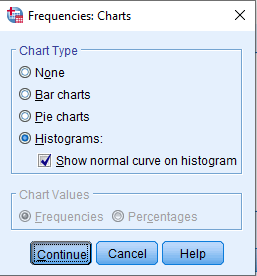
\includegraphics[width=6cm]{img/1111118}
		\caption{Click Continue}
	\end{figure}
\end{frame}
% Slide 
\begin{frame}[t]{Histograms for Scale Variables}
	\begin{figure}
		\centering
		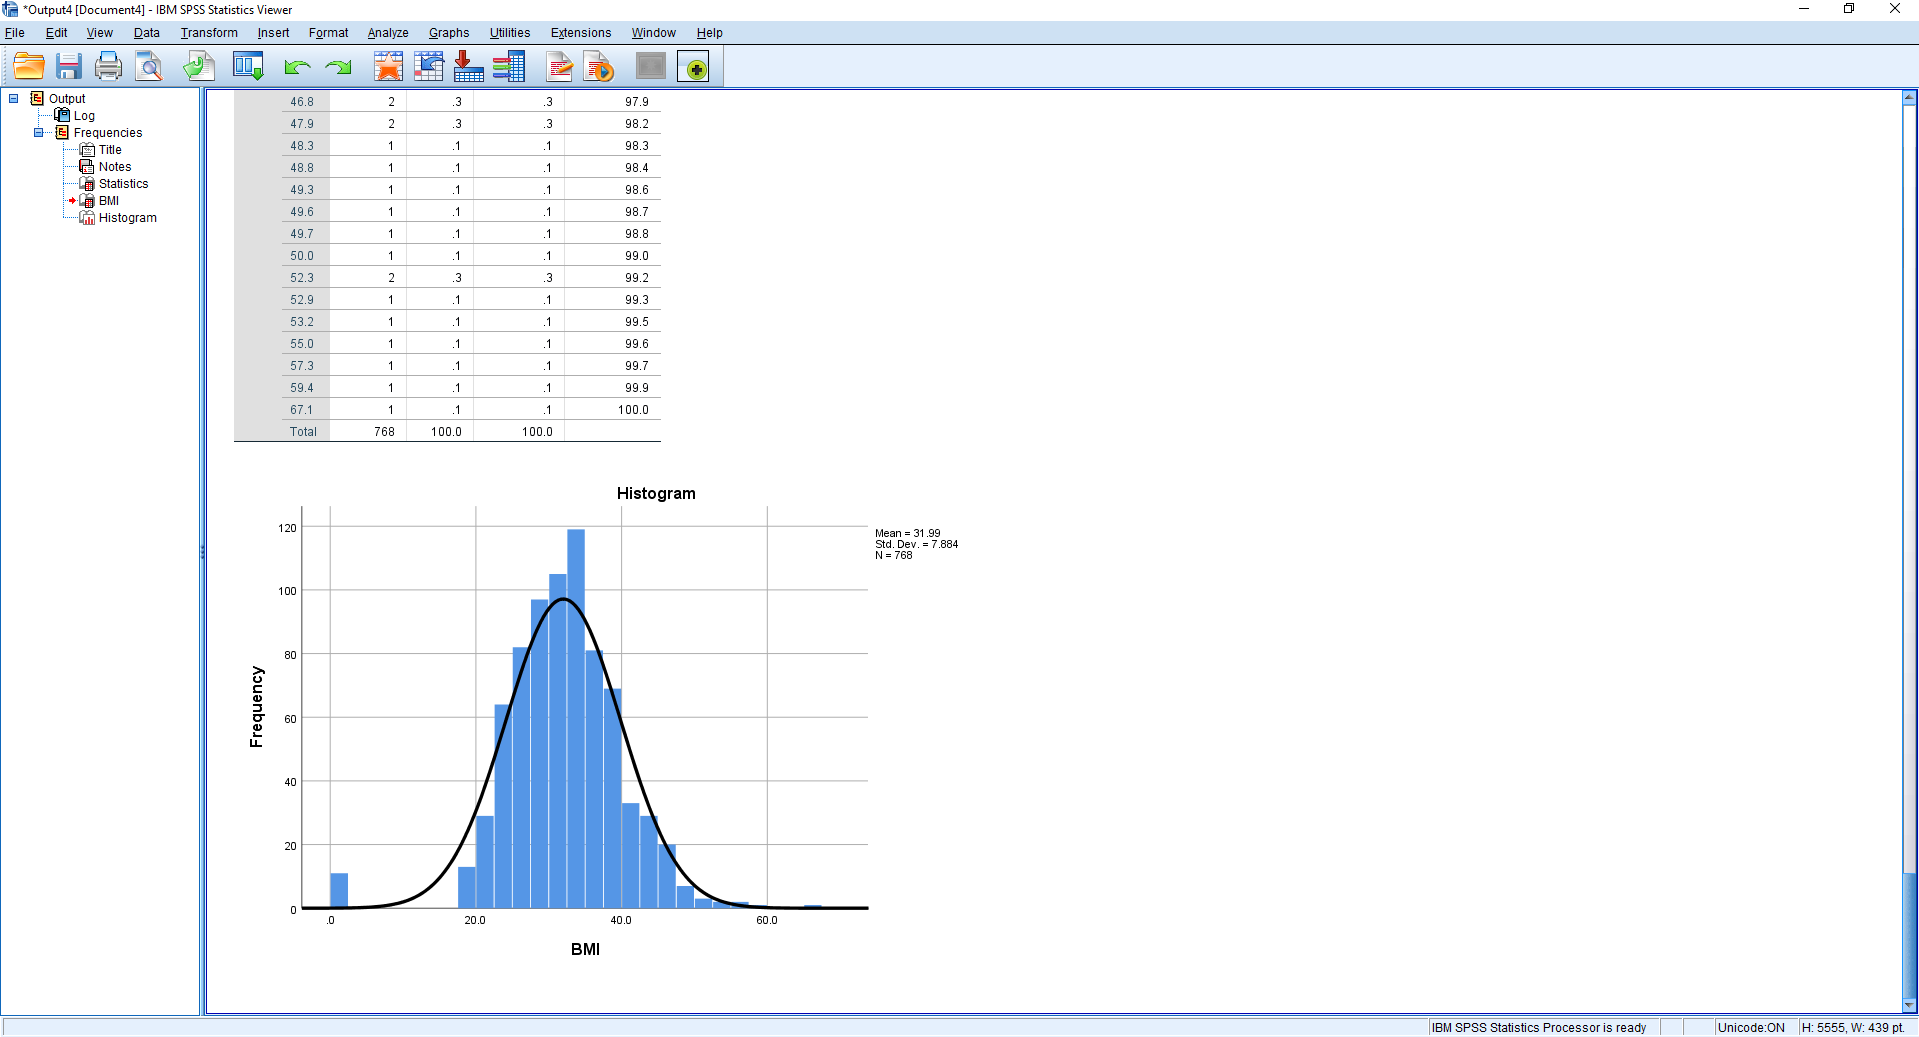
\includegraphics[width=12cm]{img/1111119}
		\caption{Histogram Result}
	\end{figure}
\end{frame}
%-----------End----------------------------------
%section-2
\section{SECTION-II Creating and Editing Charts}
%-------------------Charts for Categorical Data-------------------------
%slide
\begin{frame}[t]{Chart creation basics (Con..)}
	\begin{itemize}
		\item From the menus choose:\\
		Graphs \textgreater Graph Board Template Chooser..
		\item Click Variables.
		\item Select Charts.
		\item Click OK.
		
	\end{itemize}
\end{frame}

% Slide 
\begin{frame}[t]{Chart creation basics (Con..)}
	\begin{figure}
		\centering
		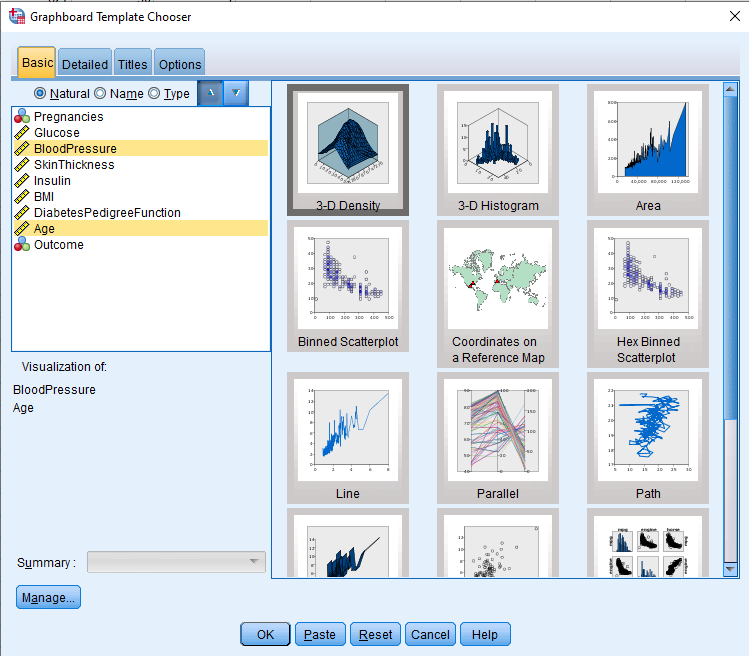
\includegraphics[width=6cm]{img/charts_2}
		\caption{Select Variables}
	\end{figure}
\end{frame}
% Slide 
\begin{frame}[t]{Chart creation basics (Con..)}
	\begin{figure}
		\centering
		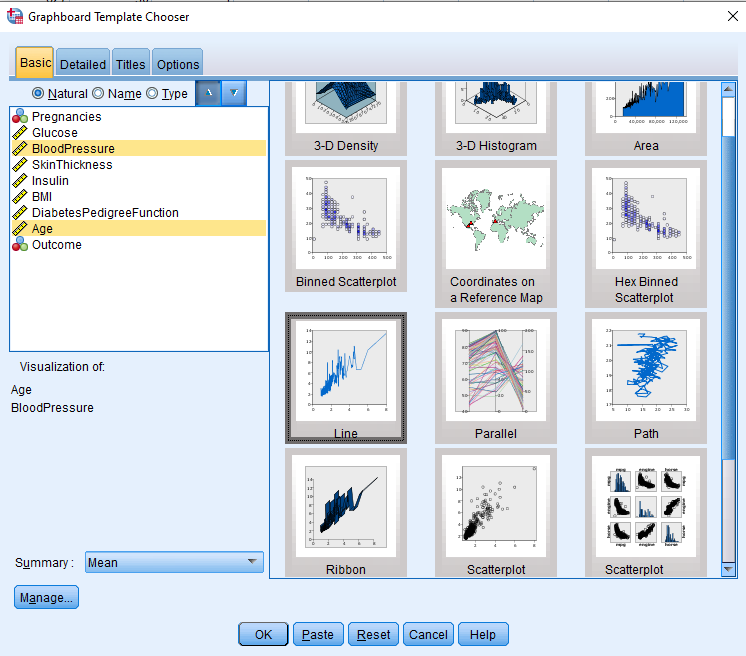
\includegraphics[width=6cm]{img/charts_3}
		\caption{Click Line}
	\end{figure}
\end{frame}
% Slide 
\begin{frame}[t]{Chart creation basics (Con..)}
	\begin{figure}
		\centering
		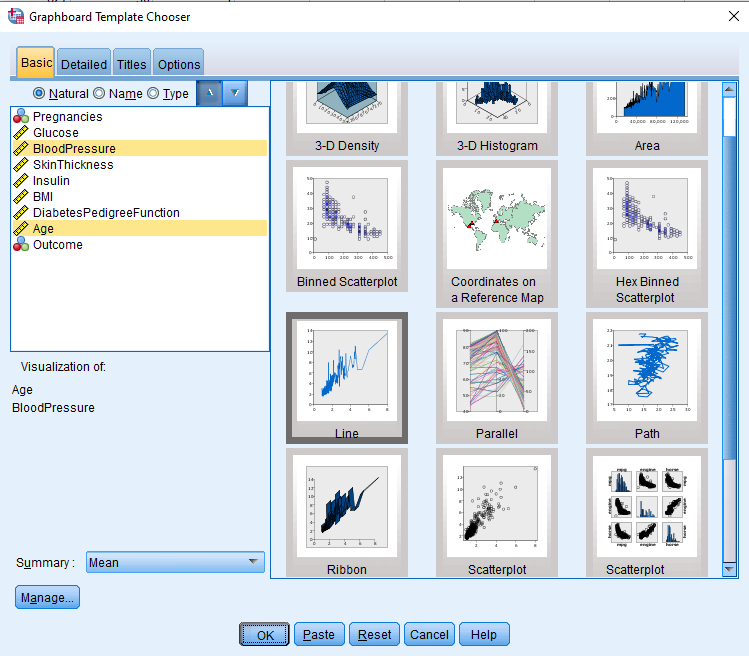
\includegraphics[width=6cm]{img/charts_4}
		\caption{Click Ok}
	\end{figure}
\end{frame}
% Slide 
\begin{frame}[t]{Chart creation basics}
	\begin{figure}
		\centering
		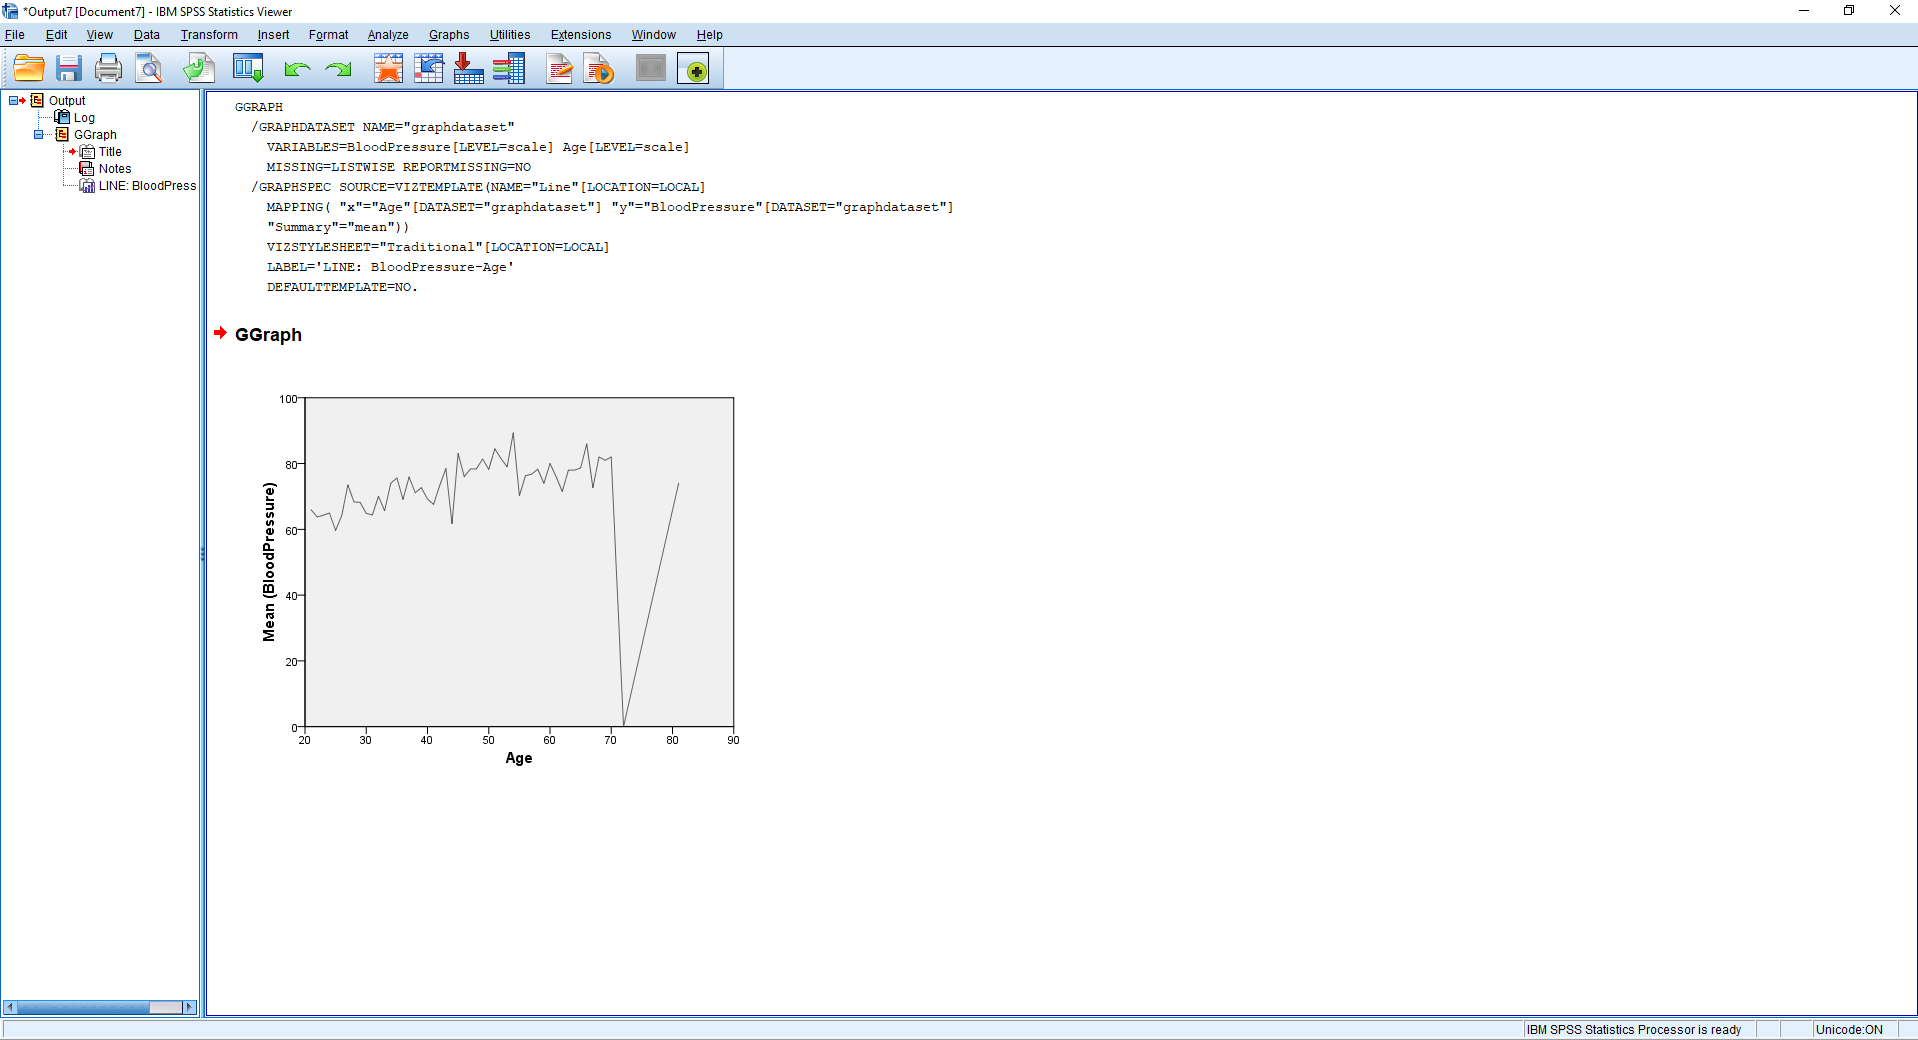
\includegraphics[width=12cm]{img/charts_5}
		\caption{Line Charts result}
	\end{figure}
\end{frame}
%-----------End----------------------------------

%----------------------Edit Charts Basic-----------------------------
%slide
\begin{frame}[t]{Chart editing basics (Con..)}
	\begin{itemize}
		\item Double Click on the Graphs.
		\item Click and \textit{Select What you want to Edit}
		\item Click Files form menu
		\item Click Close
		
	\end{itemize}
\end{frame}

% Slide 
\begin{frame}[t]{Chart editing basics (Con..)}
	\begin{figure}
		\centering
		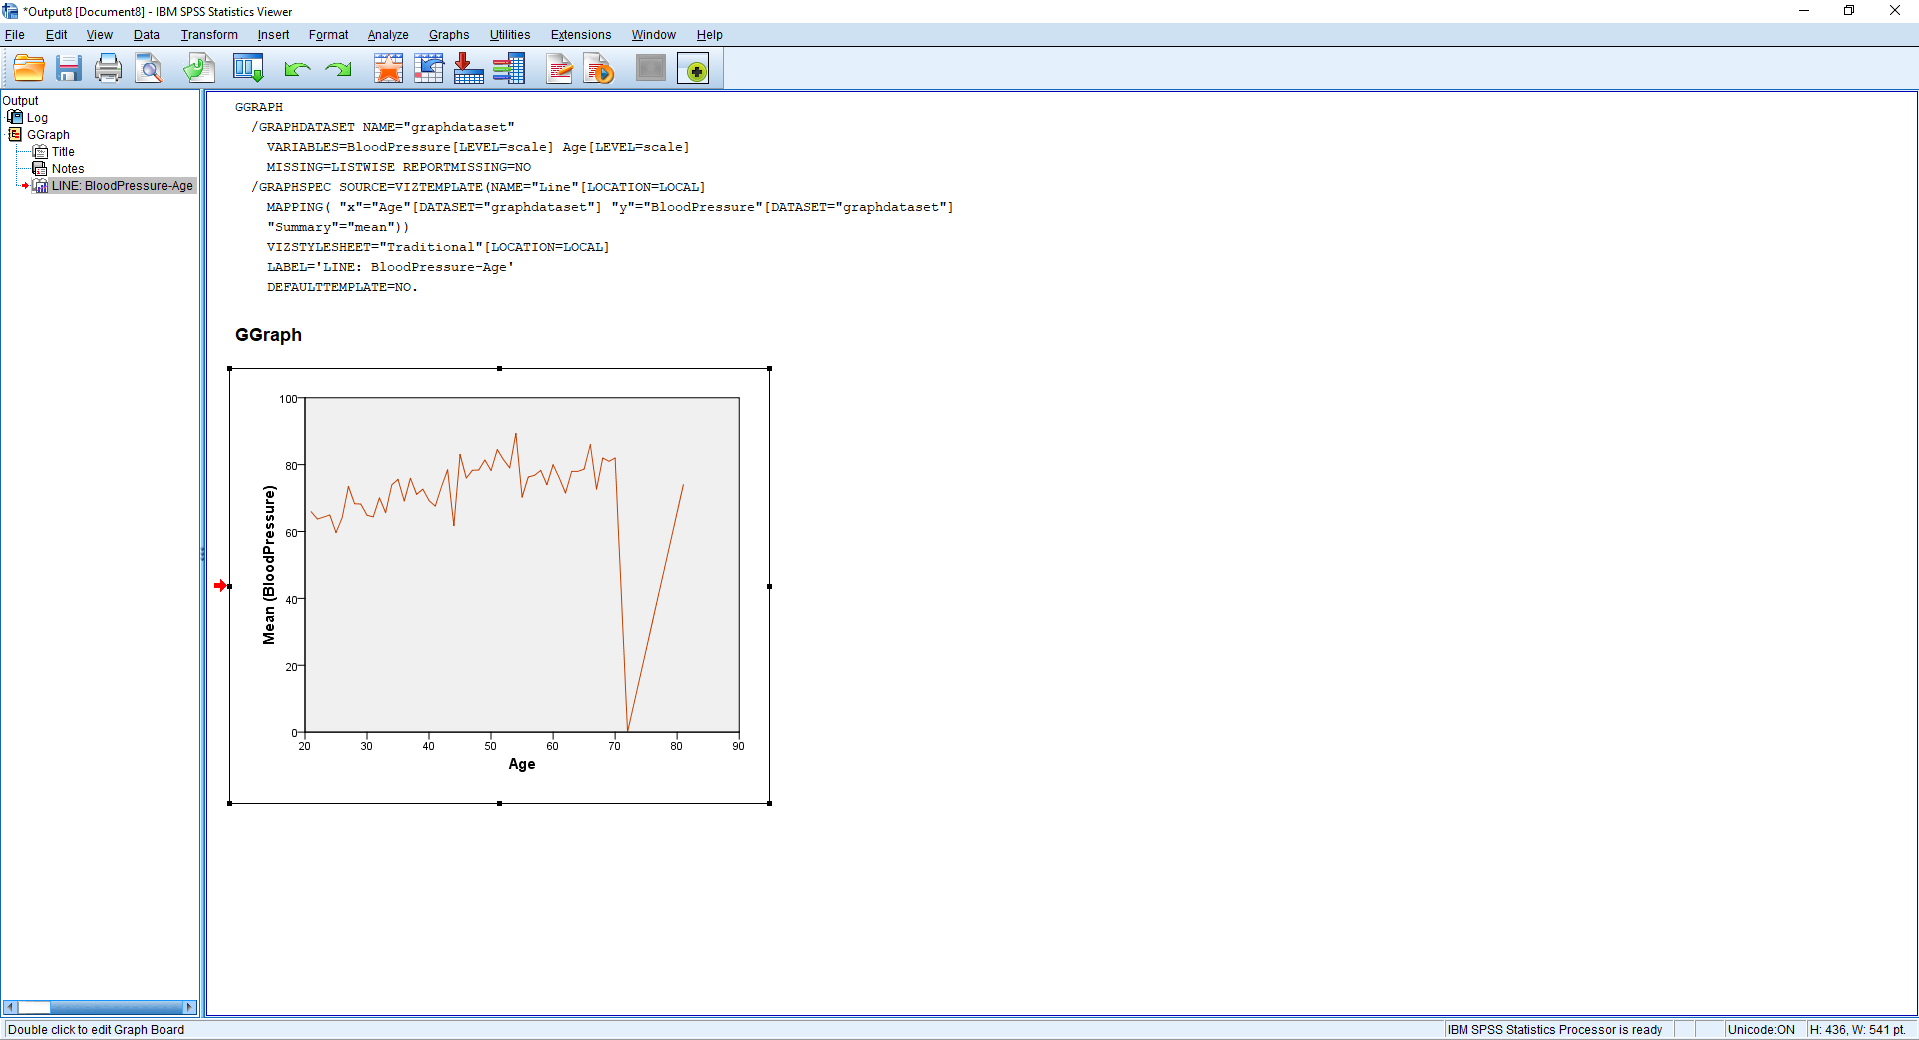
\includegraphics[width=12cm]{img/edit_chart-1}
		\caption{Double Click on the Graphs}
	\end{figure}
\end{frame}
% Slide 
\begin{frame}[t]{Chart editing basics (Con..)}
	\begin{figure}
		\centering
		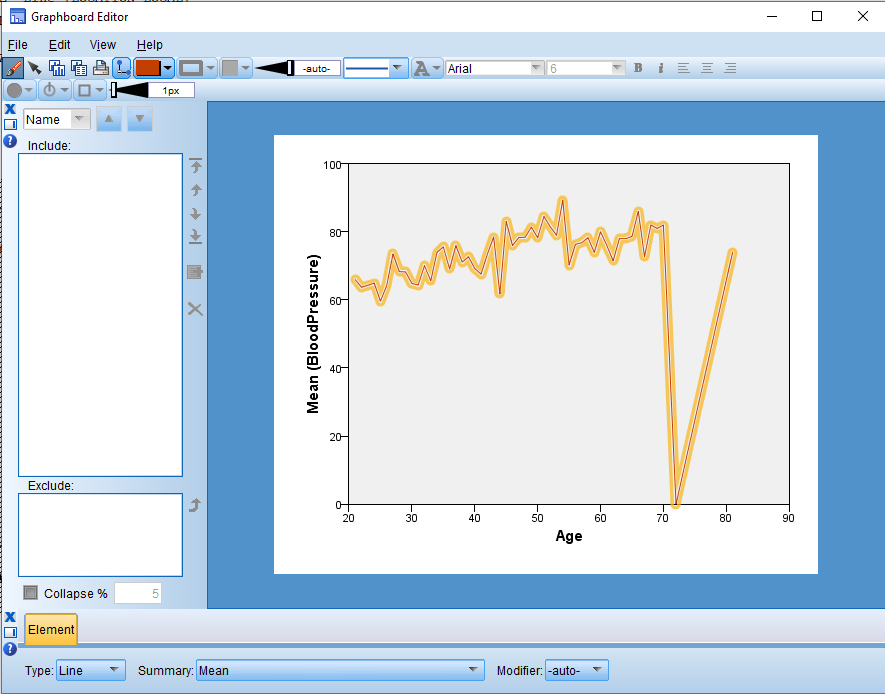
\includegraphics[width=8cm]{img/edit_chart-2}
		\caption{Click Line to edit line of the Graphs}
	\end{figure}
\end{frame}
% Slide 
\begin{frame}[t]{Chart editing basics (Con..)}
	\begin{figure}
		\centering
		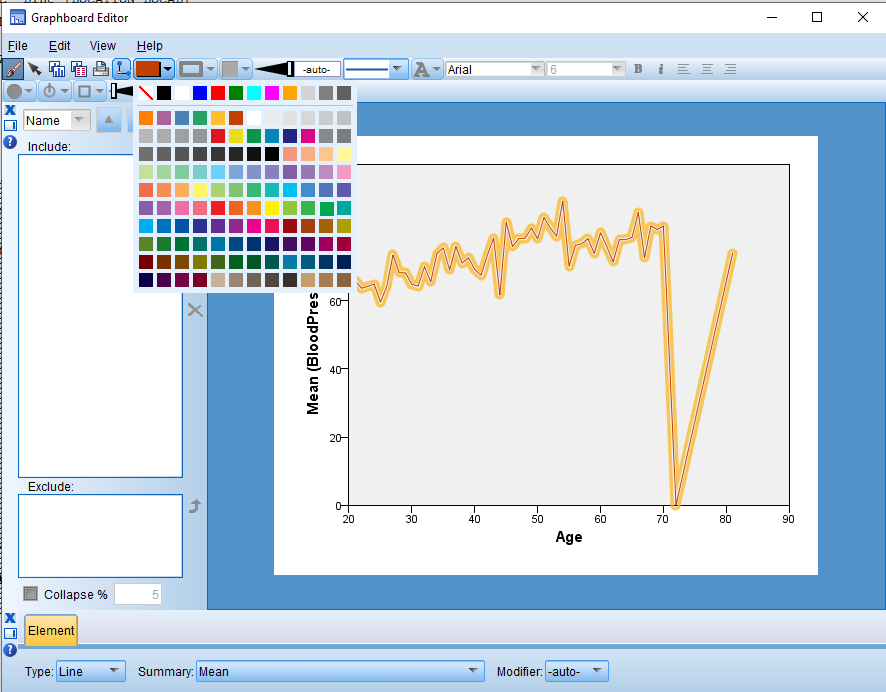
\includegraphics[width=8cm]{img/edit_chart-3}
		\caption{Change Graphs(line) color form the color palate}
	\end{figure}
\end{frame}
% Slide 
\begin{frame}[t]{Chart editing basics (Con..)}
	\begin{figure}
		\centering
		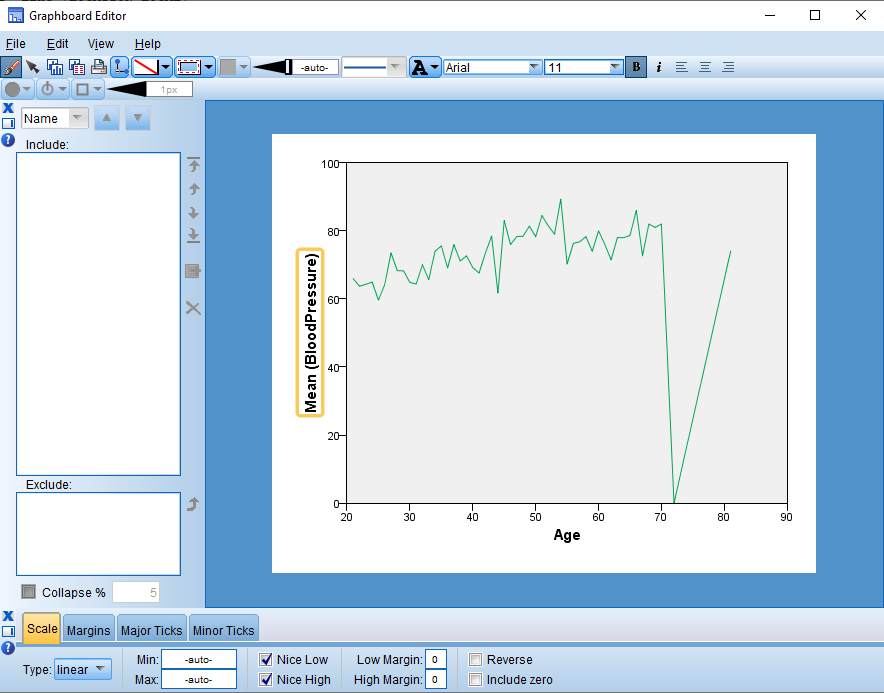
\includegraphics[width=8cm]{img/edit_chart-4}
		\caption{Select and Edit Y-axis}
	\end{figure}
\end{frame}
% Slide 
\begin{frame}[t]{Chart editing basics (Con..)}
	\begin{figure}
		\centering
		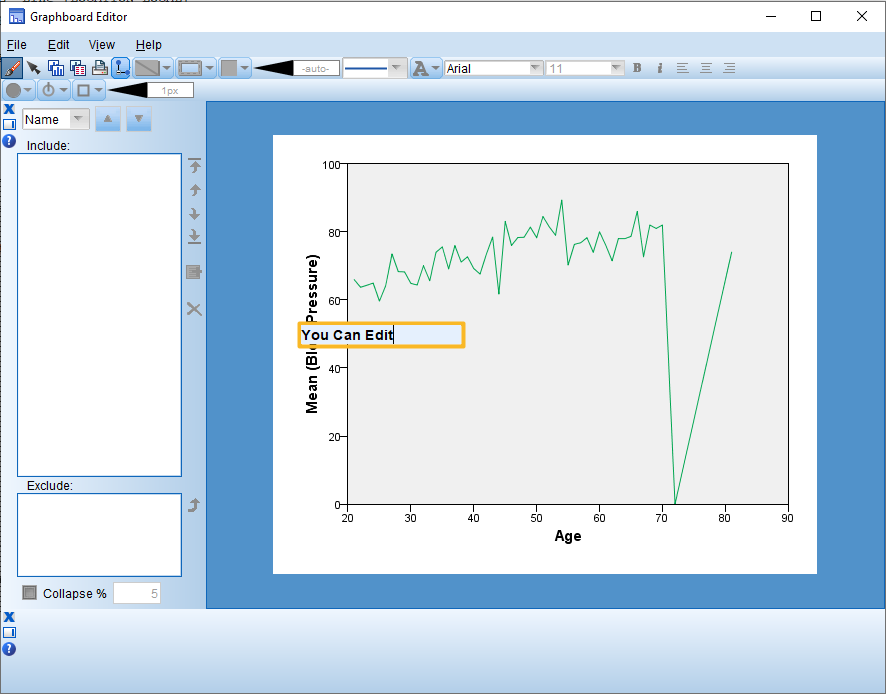
\includegraphics[width=8cm]{img/edit_chart-5}
		\caption{Write and click enter}
	\end{figure}
\end{frame}
% Slide 
\begin{frame}[t]{Chart editing basics (Con..)}
	\begin{figure}
		\centering
		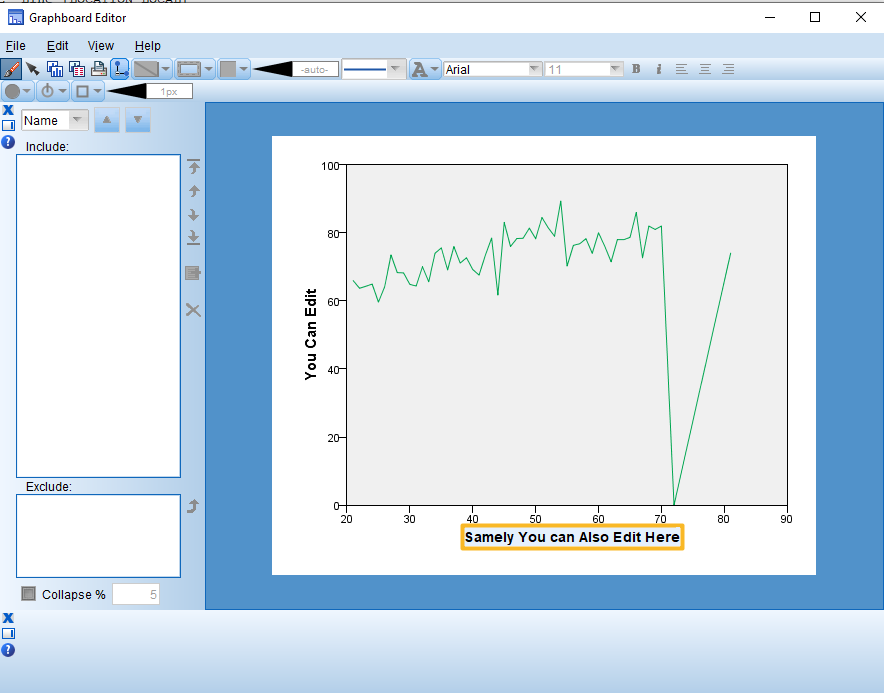
\includegraphics[width=8cm]{img/edit_chart-6}
		\caption{Select and Edit X-axis}
	\end{figure}
\end{frame}
% Slide 
\begin{frame}[t]{Chart editing basics (Con..)}
	\begin{figure}
		\centering
		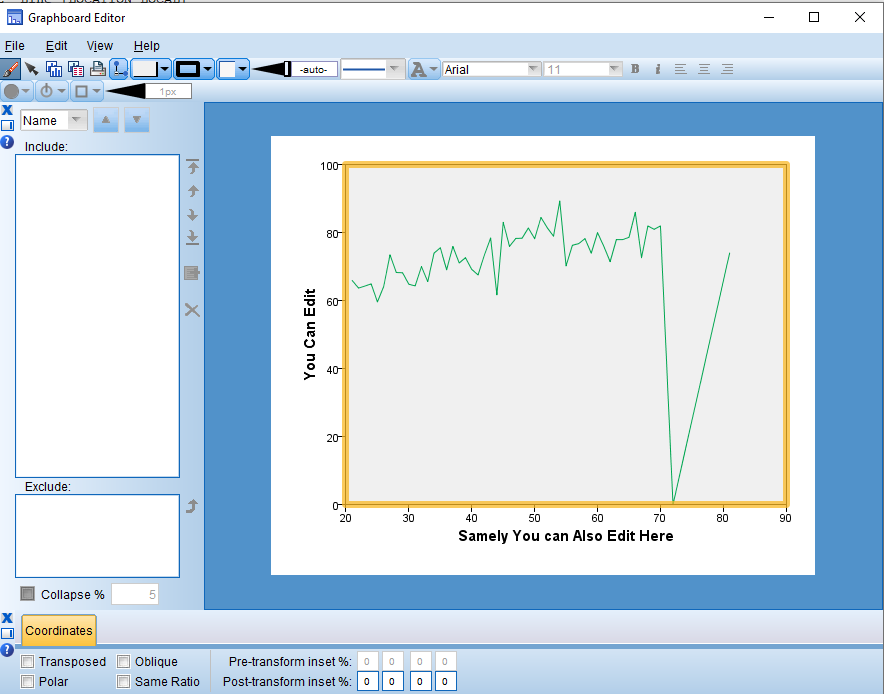
\includegraphics[width=8cm]{img/edit_chart-7}
		\caption{Click and Select Border and Background or canvas of the Graphs}
	\end{figure}
\end{frame}
% Slide 
\begin{frame}[t]{Chart editing basics (Con..)}
	\begin{figure}
		\centering
		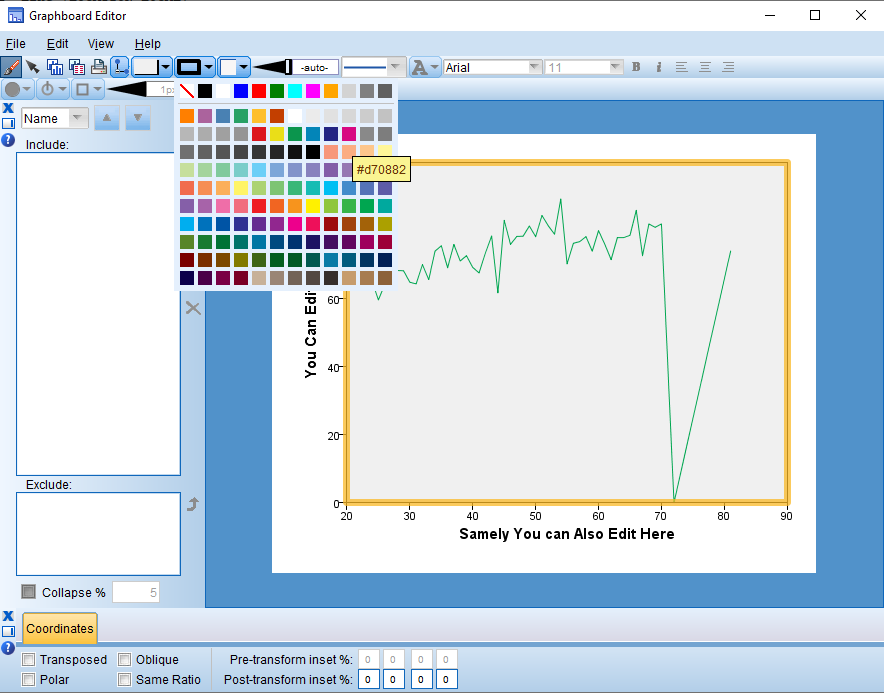
\includegraphics[width=8cm]{img/edit_chart-8}
		\caption{Change Border color form the color palate}
	\end{figure}
\end{frame}
% Slide 
\begin{frame}[t]{Chart editing basics (Con..)}
	\begin{figure}
		\centering
		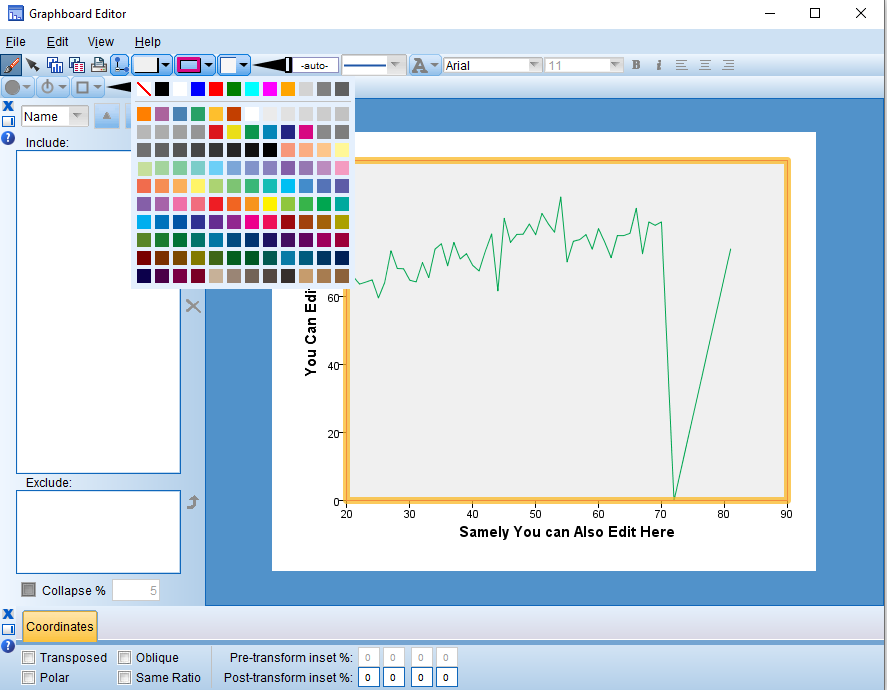
\includegraphics[width=8cm]{img/edit_chart-9}
		\caption{Change Background or canvas color form the color palate}
	\end{figure}
\end{frame}
% Slide 
\begin{frame}[t]{Chart editing basics (Con..)}
	\begin{figure}
		\centering
		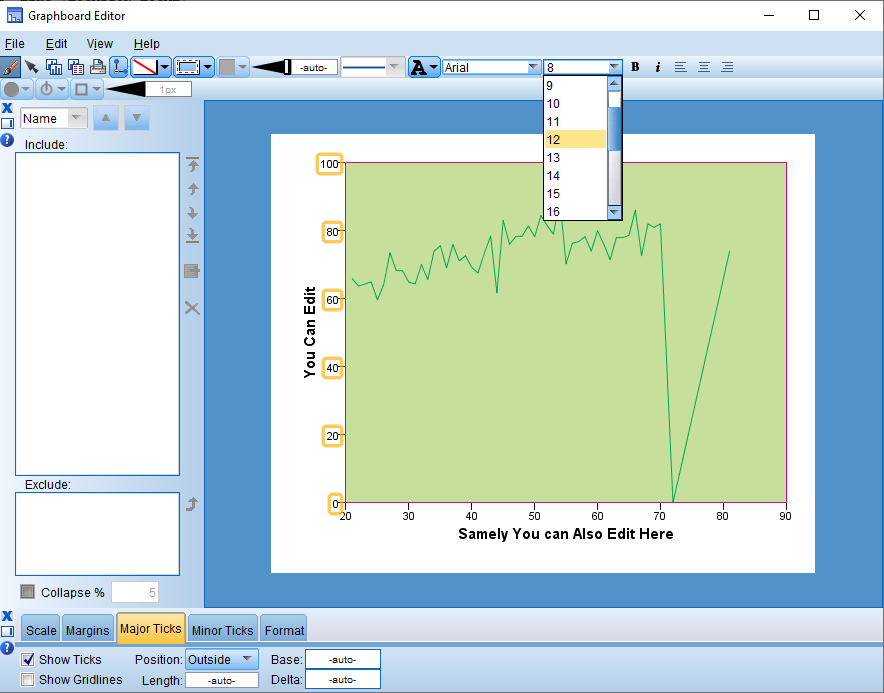
\includegraphics[width=8cm]{img/edit_chart-10}
		\caption{Click and Select Ticks of the Graph and Increase Ticks Font size}
	\end{figure}
\end{frame}
% Slide 
\begin{frame}[t]{Chart editing basics}
	\begin{figure}
		\centering
		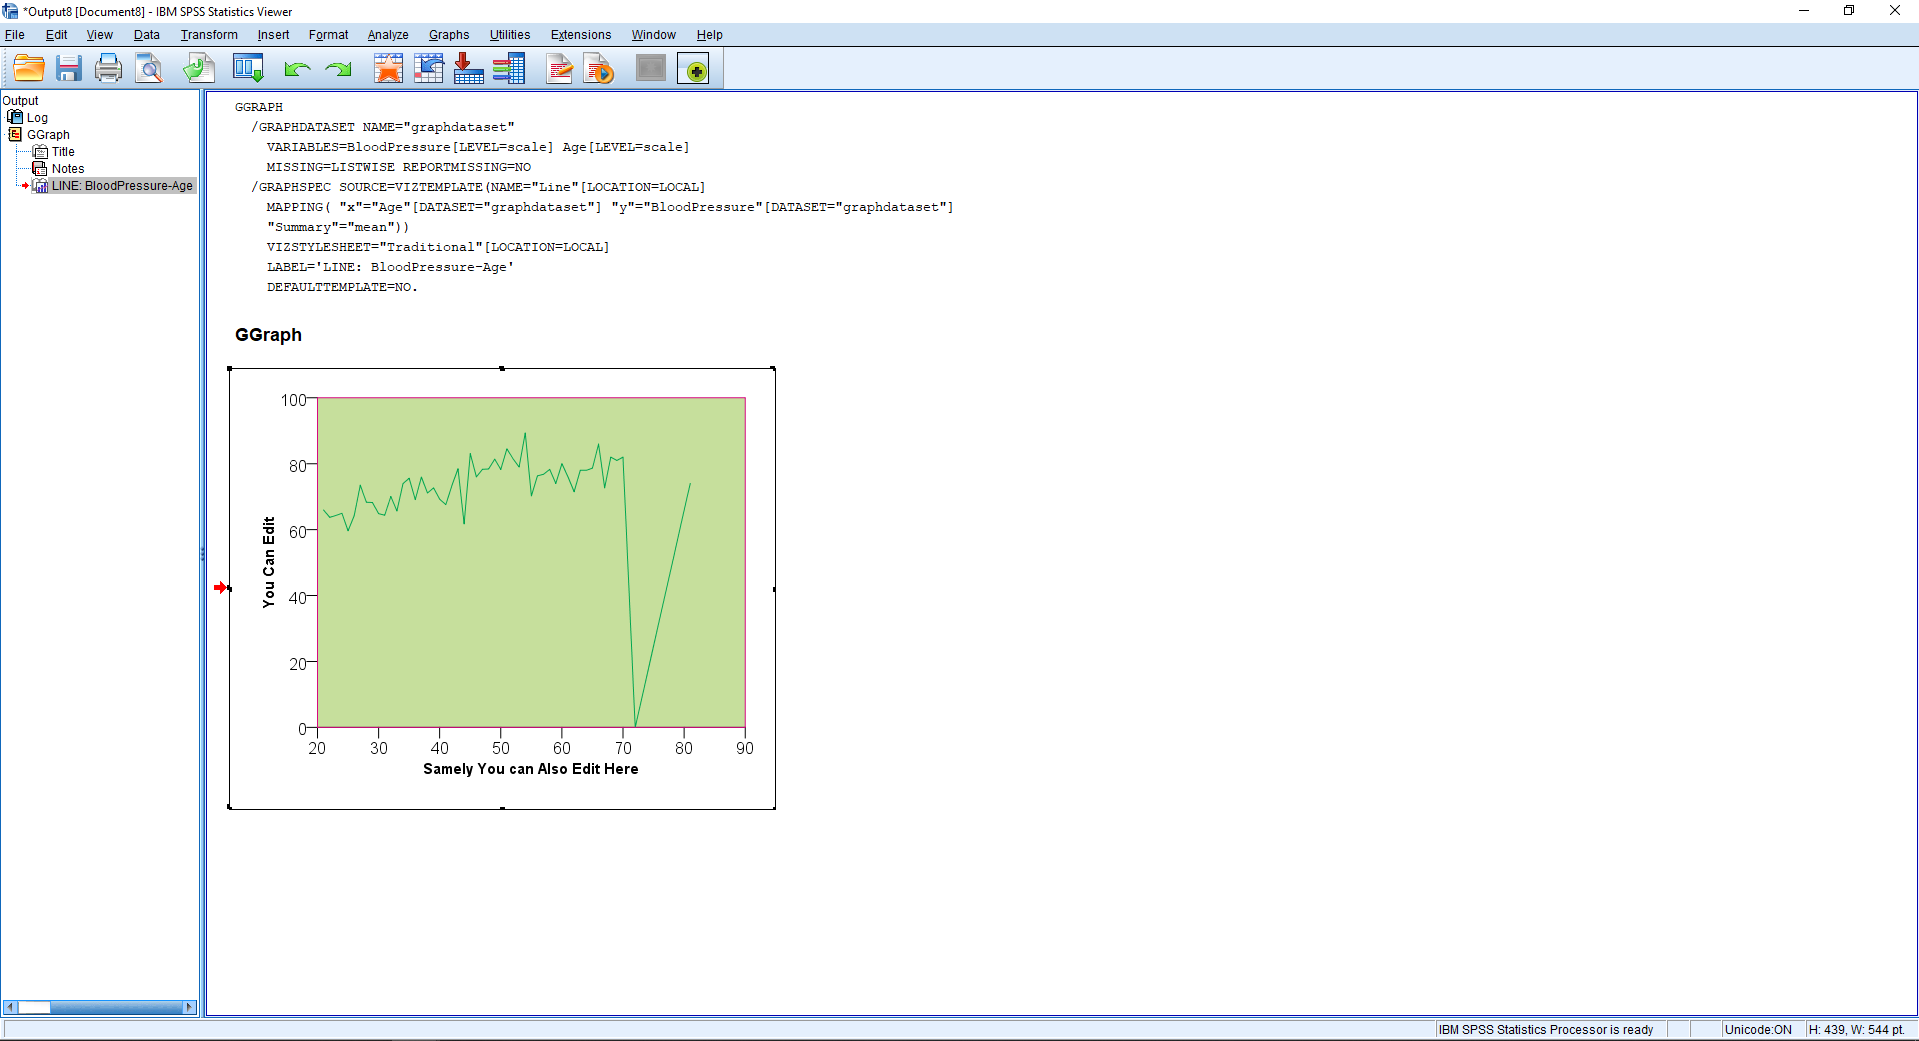
\includegraphics[width=12cm]{img/edit_chart-11}
		\caption{Edited Graphs}
	\end{figure}
\end{frame}
%-----------End----------------------------------

%---------------------Note-------------------------
\begin{frame}[t]{Table Editing Idea}
	\textbf{As we have edited the  graphs, following the same process (select and edit) we can edit the table also.}
\end{frame}









% Thank you slide 
\plain{Thank You\\ \ \\ \Huge{\smiley}}

\end{document}